\documentclass[11pt,a4paper,spanish]{book}
\usepackage{unir}

%---------------------------
% Rellenar con la información apropiada al trabajo.
%---------------------------
\title{Aplicación de algoritmos cuánticos a la conjetura de Collatz}
\titulacion{Máster en Computación Cuántica}
\author{Sergio Cardona Tárrega}
\date{\today}
\director{Francisco Costa Cano}
\nombreciudad{Valencia}

\begin{document}

\maketitle

\frontmatter
\tableofcontents
\listoffigures
\listoftables
\chapter{Resumen}

En este apartado se introducirá un breve resumen en español del trabajo realizado (extensión máxima: 150 palabras). Este resumen debe incluir el objetivo o propósito de la investigación, la metodología, los resultados y las conclusiones.

{\bf Palabras clave:} se deben incluir de 3 a 5 palabras claves en español
\titulo{Abstract}

En este apartado se introducirá un breve resumen en inglés del trabajo realizado. Este resumen debe incluir el objetivo o propósito de la investigación, la metodología, los resultados y las conclusiones.

(Aproximadamente 150 palabras)

\textbf{Keywords:} (De 3 a 5 palabras en inglés)

\mainmatter
\chapter{Introducción}

Este trabajo se centra en el desarrollo y aplicación de algoritmos cuánticos para la optimización de rutas de entrega y volumen de carga en la empresa Wolf. Utilizando técnicas de computación cuántica, se busca abordar los desafíos específicos relacionados con la eficiencia en la distribución y el aprovechamiento del espacio de carga en una flota de camiones. 

%El primer capítulo es siempre una introducción. En ella debes resumir de forma esquemática pero suficientemente clara lo esencial de cada una de las partes del trabajo. La lectura de este primer capítulo ha de dar una primera idea clara de lo que se pretendía, las conclusiones a las que se ha llegado y del procedimiento seguido.
%Como tal, es uno de los capítulos más importantes de la memoria. Las ideas principales a transmitir son la identificación del problema a tratar, la justificación de su importancia, los objetivos generales (a grandes rasgos) y un adelanto de la contribución que esperas hacer.
%Típicamente una introducción tiene tres apartados: Motivación, Planteamiento del trabajo, Estructura del trabajo. (Texto Normal del menú de estilos.)
%(Ejemplo de nota al pie\footnote{Ejemplo de nota al pie.}.)

\section{Motivación}

    El transporte y la logística son vitales para la economía global, pero enfrentan problemas significativos relacionados con la optimización de rutas y la carga de vehículos. Las soluciones actuales son a menudo ineficientes, llevando a un uso subóptimo de recursos, aumento de costos y tiempo de entrega. Este trabajo identifica y aborda estas ineficiencias utilizando algoritmos cuánticos, que prometen una capacidad superior para manejar la complejidad y dinamismo de tales sistemas.
    La importancia de optimizar rutas de entrega y carga se magnifica en contextos de alta demanda y diversidad geográfica, como lo es el caso de la empresa Wolf. Los desafíos incluyen la gestión eficiente de múltiples puntos de recolección y distribución, la variabilidad en el tamaño y volumen de los paquetes, y restricciones temporales estrictas. La computación cuántica ofrece un enfoque prometedor para superar estos retos, lo que podría resultar en una significativa reducción de costos operativos y mejora en la eficiencia del servicio.


%Cuál es el problema que quieres tratar? ¿Cuáles crees que son las causas? ¿Por qué es relevante el problema?

%A continuación, se indica con un ejemplo cómo deben introducirse los títulos y las fuentes en Tablas y Figuras.

%\begin{table}[t]
%	\begin{center}
%	\caption{Ejemplo de tabla con sus principales elementos.}
%	\label{tab:1}
%	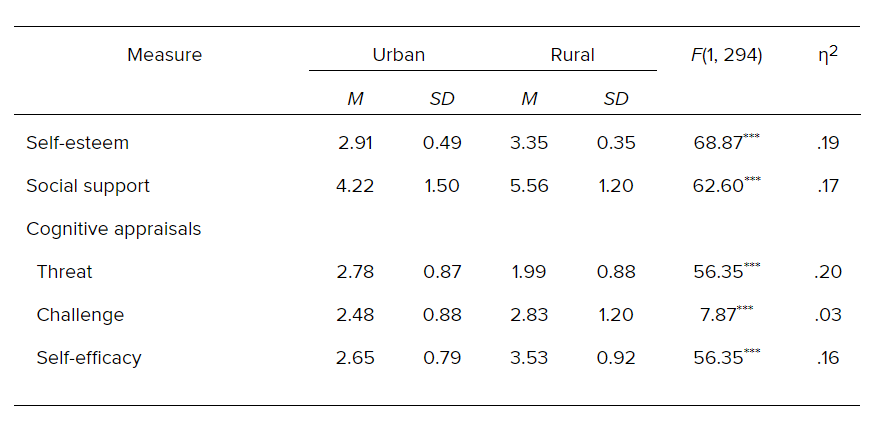
\includegraphics[width=4.90737in,height=2.42708in]{tabla}
%	\small Fuente: American Psychological Association, 2020e.
%	\end{center}
%\end{table}

%\begin{figure}[H]
%	\begin{center}
%		\caption{Ejemplo de figura realizada para nuestro trabajo.}
%		\label{fig:1}
%		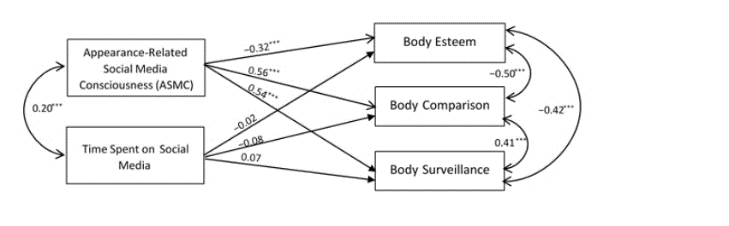
\includegraphics[width=4.90737in,height=2.42708in]{figura}
%%		\small Fuente: American Psychological Association, 2020f.
%	\end{center}
%\end{figure}

\section{Planteamiento del trabajo}

    Este estudio se centra en el desarrollo y evaluación de algoritmos cuánticos diseñados para optimizar las rutas de entrega y la carga de camiones para la empresa Wolf. Se analizarán y compararán estos algoritmos con métodos clásicos de optimización para determinar su viabilidad y eficacia. Dividiremos el probleam en tres partes específicos:

    \begin{itemize}
    \item Optimización de rutas: Desarrollar un algoritmo que mejore la eficiencia de las rutas de entrega, teniendo en cuenta la ubicación geográfica de los puntos de distribución, el tamaño y volumen de los paquetes, y los intervalos de tiempo de entrega.
    
    \item Planificación de itinerarios: Crear un sistema que detalle el tiempo estimado de llegada para cada vehículo a todos los puntos de distribución.
    
    \item Optimización de la carga: Mejorar el proceso de carga de los vehículos, ordenando los paquetes de manera que se maximice el uso del espacio disponible y se optimice la eficiencia del transporte.
    
    La investigación evaluará la aplicabilidad de varios algoritmos cuánticos, incluyendo el recocido cuántico y el algoritmo de Grover, y utilizará plataformas como IBM Quantum, D-Wave y Rigetti.
    \end{itemize}

%¿Cómo se podría solucionar el problema? ¿Qué es lo que se propone? Aquí describes tu objetivo en términos generales. 

\section{Estructura de la memoria}

    Este trabajo estará organizado en los siguientes capítulos para abordar de manera sistemática el problema de investigación:

    \textbf{Introducción:} Presentación del problema, justificación y objetivos del estudio.
    Fundamentos Teóricos: Explicación de los conceptos básicos de la mecánica cuántica y la computación cuántica necesarios para entender los algoritmos utilizados.
    
    \textbf{Metodología:} Detalle de las técnicas y herramientas cuánticas seleccionadas, así como la metodología de comparación con sistemas clásicos.
    Desarrollo de Algoritmos y Simulaciones: Diseño de los algoritmos cuánticos y realización de simulaciones para evaluar su rendimiento.
    
    \textbf{Resultados y Análisis:} Presentación y análisis de los resultados obtenidos, comparando las soluciones cuánticas con las clásicas.
    
   \textbf{ Conclusiones y Recomendaciones:} Síntesis de los hallazgos y sugerencias para futuras investigaciones o aplicaciones prácticas. 

%Aquí describes brevemente lo que vas a contar en cada uno de los capítulos siguientes.
\chapter{Contexto y estado del técnica}

Después de la introducción, se suele describir el contexto de aplicación. En este Capítulo debemos mostrar un sobrado conocimiento de la materia, plagando absolutamente TODO lo que mencionemos con referencias. Práticamente, cada frase puede necesitar de alguna referencia.

Las referencias NO están solo para aparentar. Rendimos tributo y reconocemos a las personas que han pensado los problemas antes que nosotros. Puede haber varias referencias válidas para una misma afirmación, y no pasa nada porque así se indique.

Recuerda que para citar trabajos de diferentes autores es fundamental e imprescindible seguir el formato APA, según se describe en el documento Normativa\_APA.pdf disponible en el apartado de Documentación del Aula de información general del Máster Universitario en Computación Cuántica (MUCC). No se debe mencionar, ni utilizar ninguna fuente, sin citarla apropiadamente.

EJEMPLO DE CITAS: Si queremos citar a alguien, por ejemplo porque vamos a hablar de Latex \citep{lamport1994} o porque, según las ideas de \cite{ackerman2017}, la liga de fútbol inglesa debe tener torneos de desempate, pues tenemos que hacerlo correctamente. {\bf{(Ver en la sección Bibliografía cómo deben incluirse las entradas bibliográficas).}}

Este Capítulo puede tener secciones diferentes a las que se indican a continuación, que se indican a modo de ejemplo.

\section{Antecedentes históricos}

En 1980, Paul Benioff propone la primera versión teórica de una máquina de Turing cuántica poniendo de manifiesto que la computación cuántica era, en efecto, teóricamente posible (Benioff, 1980). Poco tiempo después, Richard Feynman constató que existían ciertos fenómenos cuya simulación requería de recursos que crecían de manera exponencial con la complejidad del problema y sugirió el empleo de computadores cuánticos para simular este tipo de fenómenos (Feynman, 1982). A mediados de los 80, David Deustch describe la Máquina de Turing Universal Cuántica, probando que construir un computador cuántico era teóricamente posible (Deutsch, 1985). En este mismo artículo, aparece el algoritmo de Deutsch, el primer algoritmo que resuelve un problema de manera más eficiente que su versión clásica.

Durante la década de los 90, aparecerán dos de los algoritmos más importantes en computación cuántica. En primer lugar, el algoritmo de Shor es capaz de factorizar enteros con una ventaja exponencial respecto a los algoritmos clásicos (Shor, 1994). En segundo lugar, el algoritmo de Grover diseñado para realizar búsquedas en una base de datos no estructurada de manera más eficiente (Grover, 1996). La aparición de estos algoritmos pone de manifiesto la existencia de una ventaja cuántica en este nuevo modelo de computación.

Este nuevo paradigma no utiliza bits clásicos  si no bits cuánticos o qubits, término atribuido a Benjamin Schumacher (1995). En el año 2000, Divincenzo propone 5 requisitos que debe cumplir todo sistema para que pueda ser considerado como una implementación física válida de un computador cuántico (Divincenzo, 2000):

\begin{enumerate}
    \item Debe tratarse de un sistema escalable con al menos un qubit bien caracterizado.
    \item Debe poder inicializarse a un estado inicial, habitualmente 
    $ | 0 \rangle $.
    \item Cada qubit debe tener un tiempo de decoherencia significativamente superior a los tiempos de actuación de las puertas cuánticas.
    \item Debe poseer un conjunto universal de puertas cuánticas.
    \item Debe poseer algún mecanismo que permite medir el estado de los qubits.
\end{enumerate}










\section{Estado actual}

En la siguiente sección, se expondrán todos aquellos conceptos de la Mecánica Cuántica y, mas específicamente, de la computación cuántica de los que nos serviremos durante el desarrollo del presente trabajo.

\subsection{Postulados de la mecánica cuántica}

El formalismo matemático de la mecánica cuántica se rige por los siguientes postulados (Nielsen y Chuang, 2010):

\begin{description}
    \item[Postulado 1] Para cada sistema físico, existe un espacio vectorial complejo con producto interno (es decir, un espacio de Hilbert) conocido como espacio de estado. El estado de dicho sistema queda completamente descrito por un vector unitario perteneciente al espacio de estados. 
    
    \item[Postulado 2] El estado de un sistema evoluciona según una transformación unitaria. Es decir, sea el estado $ | \psi \rangle$ y la transformación unitaria definida por el operador unitario $U$, entonces el estado $ | \psi \rangle $ evolucionará al estado $ | \psi' \rangle = U | \psi \rangle$.
    \item[Postulado 3] Las medidas cuánticas están descritas por un conjunto $ \left \{ M_m \right \}  $ de operadores de medida donde los subíndices $m$ hacen referencia al resultado obtenido en cada medida. Si el sistema se encuentra en el estado $ | \psi \rangle $ en el instante inmediatamente anterior a la medida, entonces la probabilidad de obtener el resultado $m$ es $$ p(m)= \langle \psi | M_m^\dagger M_m | \psi \rangle $$ y el estado del sistema tras la medida será $$ \frac{M_m | \psi \rangle}{\sqrt{\langle \psi | M_m^\dagger M_m | \psi \rangle}} . $$
    \item[Postulado 4] El espacio de estados correspondiente a un sistema físico compuesto viene dado por el producto tensorial de los espacios de estados correspondientes a cada uno de los sistemas físicos que componen nuestro sistema, es decir, $$| \psi \rangle = | \psi_1 \rangle \otimes | \psi_2 \rangle \otimes ... \otimes | \psi_n \rangle .$$
\end{description}

\subsection{Qubit}

Matemáticamente, un qubit es un vector unitario perteneciente a un espacio vectorial complejo de dimensión 2 para el cual existe una base ortonormal determinada por $ \left \{ | 0 \rangle , | 1 \rangle  \right \}$ (Rieffel y Polak, 2000). Así pues, el estado de un qubit queda determinado por cualquier combinación lineal $ | \psi \rangle = \alpha | 0 \rangle + \beta | 1 \rangle $ donde $ \alpha, \beta \in \mathbb{C} $ tal que $ | \alpha |^2 + | \beta |^2=1 $.

Los vectores que forman la base $\{ |0 \rangle , |1 \rangle  \}$ vienen dados por

$$ |0 \rangle = \begin{pmatrix} 1\\ 0 \end{pmatrix}, |1 \rangle = \begin{pmatrix} 0\\ 1 \end{pmatrix}.$$

Existen ciertos estados que, debido a su recurrencia, poseen una denotación propia (Nielsen y Chuang, 2010). Estos estados son los siguientes:

$$ | + \rangle = \frac{1}{\sqrt{2}} | 0 \rangle + \frac{1}{\sqrt{2}} | 1 \rangle $$
$$ | - \rangle = \frac{1}{\sqrt{2}} | 0 \rangle - \frac{1}{\sqrt{2}} | 1 \rangle $$
$$ | i \rangle = \frac{1}{\sqrt{2}} | 0 \rangle + \frac{i}{\sqrt{2}} | 1 \rangle $$
$$ | -i \rangle = \frac{1}{\sqrt{2}} | 0 \rangle - \frac{i}{\sqrt{2}} | 1 \rangle $$

Ya que $ \langle \psi | \psi \rangle = | \alpha |^2 + | \beta |^2=1$, entonces existe $ \theta \in [0, \pi]$ tal que $ | \alpha | = cos ( \frac{\theta}{2} )$ y $ | \beta | = sen ( \frac{\theta}{2} )$. De este modo, el estado de un qubit se puede representar de la siguiente manera

$$ | \psi \rangle = cos ( \frac{\theta}{2}) | 0 \rangle + e^{i \phi} sen ( \frac{\theta}{2} ) | 1 \rangle  $$

donde $\phi \in [0 , 2 \pi)$ representa la fase relativa entre los coeficientes (Willsh, Willsh y Michielsen, 2022).

De la expresión anterior, se sigue que existe una aplicación biyectiva entre cada estado cuántico y la superficie de una esfera tridimensional de radio 1, es decir, el estado cuántico de un qubit puede representarse como un punto sobre la superficie de una esfera de radio igual a 1. Esta representación se conoce como representación sobre la esfera de Bloch (1946).



\begin{figure}[ht]
	\begin{center}
		\caption{Representación sobre la Esfera de Bloch}
		\label{fig:fig-1}
		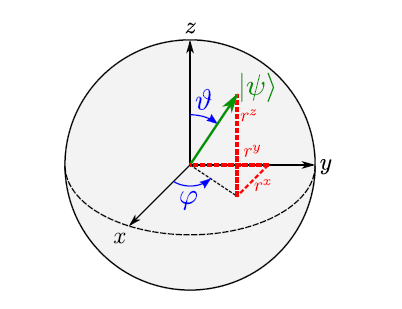
\includegraphics[width=0.5\linewidth]{Bloch.PNG}
		\small Fuente: American Psychological Association, 2020f.
	\end{center}
\end{figure}

\subsection{Medida}

En virtud del postulado 3 de la Mecánica Cuántica, existen dos resultados posibles cuando medimos el estado de un qubit, $ |0 \rangle $ o $ | 1 \rangle$. Sea el estado $ | \psi \rangle = \alpha | 0 \rangle + \beta | 1 \rangle$, entonces como resultado de una medición se obtendrá el estado $| 0 \rangle$ con una probabilidad $ | \alpha|^2$ y el estado $ | 1 \rangle $ con una probabilidad $ | \beta |^2$.

Una importante característica de las medidas cuánticas es que el estado inmediatamente anterior a la medida es destruido y sustituido por el resultado obtenido en la medida. Veamos qué implicaciones tiene esto para la cantidad de información que puede codificarse sobre un único qubit.

Como hemos visto anteriormente, cada estado cuántico se corresponde con un único punto sobre la esfera de Bloch. Dado que la superficie de la esfera tiene infinitos puntos cabría esperar que, en principio, cualquier cantidad de información pudiera ser codificada en un único qubit. No obstante, es necesario prestar atención a la naturaleza intrínseca de las medidas cuánticas ya que solo dos resultados posibles pueden producirse. Dicho de otro modo, de un único qubit mediante una medida, únicamente puede obtenerse un bit de información clásica de su estado (Nielsen y Chuang, 2010).

Otra cuestión interesante respecto a las medidas cuánticas es que pueden realizarse respecto a cualquier a base ortonormal del espacio de Hilbert. Por ejemplo, si se mide un qubit respecto de la base $\{ |+ \rangle, | - \rangle \}$, conocida como base de Hadamard, entonces los posibles resultados serán los estados $ | + \rangle$ y $ | - \rangle $. De esto, se deduce que la superposición cuántica es un fenómeno relativo a la base utilizada. Es decir, si se mide el estado $| + \rangle $ respecto de la base computacional $\{ |0 \rangle, | 1 \rangle \}$, se obtendrá el estado $ | 0 \rangle $ con un 50 $ \% $ de probabilidad o el estado $ | 1 \rangle $ con otro 50 $ \% $ de probabilidad. Queda claro que el estado $ | + \rangle $ encarna una superposición uniforme respecto de la base computacional. Del mismo modo, si se mide el estado $| 1 \rangle $ respecto de la base de Hadamard $\{ |+ \rangle, | - \rangle \}$, se obtendrá el estado $ | + \rangle $ con un 50 $ \% $ de probabilidad o el estado $ | - \rangle $ con otro 50 $ \% $ de probabilidad. Se deduce que el estado $ | 1 \rangle $ presenta una superposición uniforme respecto de la base Hadamard.


\chapter{Objetivos}
Como ya hemos mencionado dividiremos el trabajo en dos enfoques diferentes.

\section{Uso de Algoritmo de Shor para la búsqueda de ciclos de Collatz}

En el primer enfoque trataremos de utilizar la parte cuántica del algoritmo de Shor para desarrollar un algoritmo híbrido (con una parte clásica y una parte cuántica similar a la de Shor), que busque determinados ciclos de Collatz para hallar así un contraejemplo de la conjetura.

Utilizaremos además resultados sobre la conjetura de Collatz para agilizar este algoritmo, como por ejemplo el hecho de que los ciclos han de ser de determinada manera dada por \ref{RestriccionLongitudCiclo} o el hecho de que los $k-ciclos$ no existen si $k\leq91$ como se puede ver en \cite{hercher2023collatzmcycles}


\section{Uso de la representación binaria en superposición}
Para el segundo enfoque usaremos $q$ qubits para representar una superposición de todos los números desde el $0$ hasta el $2^q - 1$ en su forma binaria, en la que cada qubit en estado $|0\rangle$ o $|1\rangle$ representará que su correspondiente dígito binario es $0$ o $1$.

por ejemplo el estado $|1011\rangle$ representaría al número binario $1011$ ($11$).
$\\$

Utilizaremos la ventaja cuántica de la superposición, aplicando una puerta Hadamard a cada qubit y después trataremos de desarrollar un circuito cuántico que aplique $p$ iteraciones para comprobar finalmente que hemos alcanzado el estado correspondiente al número $1$, lo cual significará que todos los números de $q$ dígitos binarios (menores a $2^q$), verifican la conjetura.

Para ello necesitaremos qubits auxiliares y una elección de $q$ y $p$ adecuados.
$\\$

Este enfoque tiene dos principales inconvenientes.

El primero de ellos es la imposibilidad que tenemos en la computación cuántica de leer el estado del circuito sin que colapse, por lo tanto tendremos agenciárnoslas para determinar cuando el estado es $1$ y cuando es una superposición del estado $1$ con otro estado.
Para ello deberemos medir el estado y ejecutar el algortimo varias veces (y teniendo en cuenta el ruido), o bien utilizar alguna técnica para estimar el estado.

El segundo inconveniente es que los algoritmos que desarrollemos tendrán una gran cantidad de puertas cuánticas y deberemos compactar el algoritmo en gran medida (utilizando quizás más qubits auxiliares) y teniendo siempre en cuenta que es posible que la ventaja cuántica que nos ofrecen estos posibles algoritmos quede contrarrestada por el crecimiento no lineal de puertas cuánticas.


\section{Análisis de resultados}
Analizaremos los resultados de ambos enfoques primero en simulador y después en un entorno real de pocos qubits para ver como sería aplicar el proceso a gran escala cuando contemos con ordenadores cuánticos de un mayor número de qubits.

También analizaremos si merece la pena usar los algoritmos desarrollados en ambos enfoques y si podrían resultar a ser una ventaja respecto a sus posibles contrapartes clásicas a grandes escalas de cantidad de qubits (probablemente con la cantidad de qubits en los que trabajemos no lo sean). 
\chapter{Desarrollo del trabajo}


\section{Algoritmo de Shor para buscar k-ciclos}

Como ya sabemos, el algoritmo de Shor nos permitiría una eficiencia mayor a la hora de calcular el periodo de la función $2^x \equiv 1 \pmod N$, lo que nos permitiría realizar la búsqueda de ciclos de una mayor longitud.



\subsection{Breve introducción del algoritmo de Shor}
(buscar referencias y hacer una introducción al algoritmo de Shor)



\subsection{Idea general}

Como podemos ver en la fórmula de los k-ciclos \ref{FormulakCicloCollatzAlterna}, para un k-ciclo obtenemos $k$ fracciones con denominador $N=2^L-3^X$ y cuyos numeradores son $2^{y_i} - 1$ multiplicados por un respectivo factor que podemos llamar $F_i = 3^{X - X_i} 2^{L_{i-1}} 2^{x_i}$.
$\\$


De esta manera, después de calcular nuestro $r$ de forma que $2^r \equiv 1 \pmod N$, si pudiéramos encontrar los $k$ términos $y_i$ de forma que fueran múltiplos de $r$, entonces habríamos encontrado automáticamente un k-ciclo y por tanto un contraejemplo de la conjetura, demostrando su falsedad.
$\\$


De todas formas, no debemos olvidar que el hecho de no encontrar k-ciclos no probaría nada, ni siquiera la inexistencia de estos k-ciclos, pues podría existir un k-ciclo cuyo denominador $N$ no dividiera a alguno de sus numeradores (o a ninguno), y sin embargo si dividir al producto $\sum\limits_{i=1}^k F_i (2^{y_i} - 1)$. 
$\\$

Lo que haremos pues, será iterar sobre la longitud del k-ciclo $L$, Utilizaremos que $Y \approx \frac{L}{1+log_2(3)}$ y que $X \approx log_2(3) Y$ para obtener $X$ e $Y$ redondeando la expresión al número entero más cercano.
$\\$


En cada iteración de $L$, buscaremos el periodo $r$ (que podremos buscar de forma más eficiente si utilizamos la parte cuántica del algoritmo de Shor), y comprobaremos si $r$ divide a $Y$, puesto que nos interesa buscar $y_1$, $y_2$, ... múltiplos de $r$ (y recordemos que $Y=y_1+y_2+...+y_k$)
$\\$


Utilizaremos también algunas restricciones para optimizar el proceso.



\subsection{Restricción de la longitud de los ciclos}
Sabemos gracias a (\cite{LowerBoundsCycleLength}) que la longitud de un ciclo cualquiera debe ser de la forma:

$$L = 301994a + 17087915b + 85137581c$$

con $a,b,c \in \mathbb N$  y  $ac=0$
$\\$


Dicho de otra forma, la longitud de un ciclo sólo puede ser de dos formas:
$$L = 301994a + 17087915b$$
$$L = 17087915b + 85137581c$$

Por tanto, en lugar de iterar directamente sobre $L$ ($L=1, L=2,...$), podemos iterar simultáneamente en un bucle doble sobre $b=1,2,...$ y sobre $a=0,1,...$ y $c=0,1,...$ cubriendo así todos los $L$ posibles.
$\\$

Por ejemplo si $a=1$, $b=1$, obtendríamos $L=17.389.909$.

Después calcularíamos $Y = L \frac{1}{1+log_2 3}$

Luego $X = log_2 3 Y = L \frac{log_2 3}{1+log_2 3}$
$\\$


Esto desde luego nos permitiría optimizar mucho nuestro código, ya que estamos descartando muchas longitudes de ciclos que sabemos que no pueden existir debido a (\cite{LowerBoundsCycleLength}).


\subsection{Restricción sobre la dimensión $k$ de un k-ciclo}
Utilizaremos también el hecho de que no existen k-ciclos con $k \leq 91$ (\cite{hercher2023collatzmcycles}).

Esto significa que habrán al menos $92$ variables $y_i$ que necesitarán ser múltiplo de $r$.

como todas las $y_i$ deben ser múltiplos de $r$, entonces $Y=\sum\limits_{i=0}^s y_i$ deberá ser también múltiplo de $r$, por tanto eso nos restringe los posibles valores de $Y$.
$\\$


Lo que ocurrirá normalmente, y que nos impedirá encontrar k-ciclos, será que $r$ no dividirá a $Y$, de hecho será probablemente mayor.
$\\$


Encontrar un $r$ que divida a nuestro $Y$ es pues el primer paso, que nos permitirá descartar la mayoría de iteraciones sin necesidad de proseguir con el algoritmo.

En caso de que encontráramos un $r$ que sí dividiera a nuestro $Y$, tendríamos que proseguir, verificando que divida a cada uno de los $y_i$, ya que por ejemplo en un 2-ciclo podríamos obtener $r=4$, $Y=8$ pero $y_1 = 3$ y $y_2 = 5$ (aunque sepamos $k=2$ no es un ciclo posible, se entiende el ejemplo).







\subsection{Algoritmo clásico para la búsqueda del periodo}
Un algoritmo clásico en python para el cálculo del periodo podría ser el siguiente:

\begin{verbatim}
#Esta funcion busca el menor r>0 que verifica 2^r=1 (mod N) y que sea menor que Y
#Devolvera 0 si no existe y r>0 si existe
def CalculoPeriodoClasico(N, Y, debug = False):
    r=0
    mod = 1; #Comenzamos para almacenar la congruencia módulo de los respectivos 2^i
    if debug:
        print ("N:", N)
        print ("Y:", Y)
        
    #Si N es multiplo de 2 no tiene sentido seguir,
    #nunca encontraremos r>0 tal que 2^r=1(mod N)
    if (N%2 == 0):
        return 0
    
    for i in range(1, Y):
        #Multiplicamos por 2 para obtener el siguiente 2^i
        mod = mod*2
        if mod>N:
            #Como estamos multiplicando por 2, como maximo solo supera,
            #a N una vez, es decir mod<2N
            #Por lo tanto esto es análogo a hacer mod%N pero más rapido
            mod = mod - N
        if debug:
            print (i, ": ", mod)
        if mod == 1:
            #Cuando obtenemos 2^i = 1 mod N devolvemos el indice i
            return sp.Integer(i)
    
    #Si hemos acabado el for y no ha encontrado r devolvemos 0
    return 0
\end{verbatim}

En este algoritmo (seguro que se puede optimizar), nos detenemos si llegamos a $Y$, puesto que si $r>Y$ entonces nunca será múltiplo, de hecho podríamos optimizar el algoritmo comprobando simplemente los divisores de $Y$ por ejemplo.

Incluso podríamos utilizar también la restricción de que $s\geq92$ para iterar únicamente sobre los divisores de $Y$ menores de $\frac{Y}{92}$, ya que se deberá verificar que al menos $92$ valores de $y_i$ deberán ser múltiplos de $r$.

Aunque realmente con la restricción de $\sqrt{Y}$ (el mayor divisor distinto de $Y$) estaríamos restringiendo más que con $\frac{Y}{92}$ en prácticamente todos los casos de interés, puesto que trabajaremos con valores de $Y$ grandes (mucho mas que $92^2$)



\subsection{Algoritmo cuántico para la búsqueda del periodo}
Introducir aquí la implementación de la parte cuántica de Shor



\subsection{Algoritmo de búsqueda de k-ciclos}
Definimos primero una función que calcule el periodo de forma cuántica o clásica en función de una variable booleana:

\begin{verbatim}
def CalculoPeriodo(N, Y, esCuantico = False, debugPeriodo = False):
    if esCuantico:
        return CalculoPeriodoCuantico(N, Y, debugPeriodo)
    else:
        return CalculoPeriodoClasico(N, Y, debugPeriodo)
\end{verbatim}
$\\$


Ahora definimos una función para buscar los ciclos de una determinada longitud L:

\begin{verbatim}
#Esta funcion busca k-ciclos de longitud L
def BuscarCiclo(L, debug = False, debugPeriodo = False):
    #Establecemos este numero grande para debuggear N grande
    sys.set_int_max_str_digits(10000000)
    
    #Guardamos la constante log2(3) (la usaremos constantemente)
    log23 = np.log2(3)
    #Guardamos esta constante mediante la cual calculamos Y: (Y = Kly * L)
    Kly = 1/(1+log23) 
    
    #Mostramos L:
    if debug:
        print("L: ", L)
        
    #Calculamos Y en función de nuestro L
    Y = round(Kly * L) 
    #Mostramos Y:
    if debug:
        print("Y: ", Y)
        
    #Calculamos X en función de Y (que a su vez esta en función de L)
    X = round(log23 * Y)
    #Mostramos X:
    if debug:
        print("X: ", X)
        
    #Calculamos N = 2^L - 3^X
    N = pow(2,L) - pow(3,X)
    #Mostramos N:
    if debug:
        print("N: ", N)

    
    #Calculamos el periodo de con la función CalculoPeriodo
    r = CalculoPeriodo(N, Y, False, debugPeriodo) 
    
    #Mostramos el periodo obtenido (r=0 significa periodo no valido,
    #bien porque N es multiplo de 2 o porque se ha superado el limite (Y)
    if debug:
        print("r:", r)
        
    #Comprobamos que r divida a Y (y no sea 0)
    if r!=0:
        print ("r>0!")
        if Y%r == 0:
            if BusquedaYi(r, Y):
                print ("¡¡¡¡¡CICLO ENCONTRADO!!!!!")
                
    return(r)
\end{verbatim}
$\\$


La función BusquedaYi(r, Y) se encargaría de buscar una combinación válida de $y_i$ que sean múltiplos de $r$ y cuya suma sea $Y$.
$\\$

Por último buscamos todos los ciclos que verifiquen la condición $$L = 301994a + 17087915b$$ o bien $$L = 17087915b + 85137581c$$
\begin{verbatim}
#Buscamos primero el ciclo en que a=0, c=0:
BuscarCiclo(17087915, True, False)

for i in range(1, 1001):  #Iteramos la variable a entre 1 y 1000 incluidos
    for j in range (1, 1001):  #Iteramos la variable b entre 1 y 1000 incluidos
        #Buscamos k-ciclos con longitud L teniendo c=0
        L = 301994 * i + 17087915 * j  
        BuscarCiclo(L, True, False)
        #Buscamos k-ciclos con longitud L teniendo a=0
        L = 85137581 * i + 17087915 * j 
        BuscarCiclo(L, True, False)
\end{verbatim}




\section{Algoritmo Cuántico usando la representación binaria}

Utilizando la representación binaria de un número $n \in \mathbf{N}$, podemos realizar una aplicación de la función de Collatz $T$ (\ref{T(n)}), de la siguiente manera:

Si el último dígito del número binario es $0$, entonces lo eliminamos ya que el número es par y quitarlo equivale a dividir entre $2$.

Si por el contrario el último dígito es $1$ eso significa que el número es impar y lo que hacemos es añadirle un $1$ al final (obteniendo $2n+1$) y sumarlo al número original (obteniendo $3n+1$).
Sabemos por supuesto que ese número será par y acabará en $0$, por tanto por último eliminaremos el último dígito para así obtener finalmente $\frac{3n+1}{2}$.
$\\$

Veámoslo con un ejemplo pequeño:

Si $n=11$, tenemos la sucesión $\{11, 17, 26, 13, 20, 10, 5, 8, 4, 2, 1,...\}$ que evidentemente alcanza el número $1$.

Escribimos $n$ en binario: $1011$.

Ahora como es impar, sumaríamos $1011$ y $10111$ y eliminaríamos el último $0$ obteniendo: $10001$ (que es nuestro $17$).

De nuevo es impar así que sumamos $10001$ y $100011$ y eliminamos el último $0$ obteniendo $11010$ ($26$).

Ahora es par, así que eliminamos un $0$ adicional obteniendo $1101$ ($13$).

De nuevo impar, sumamos $1101$ y $11011$ eliminando el último $0$ y obtenemos ahora: $10100$ ($20$).

Ahora $10100$ no solamente es par, si no que además es divisible entre $4$ (tiene dos $0$ al final), así que podemos quitarlos directamente (esto equivaldría a realizar el paso de quitar el último $0$ dos veces).

Obtenemos $101$ ($5$) por tanto sumamos $101$ y $1011$ obteniendo $1000$ ($8$).

Y ya llegaríamos finalmente a $1$ después de eliminar los $3$ últimos ceros.


\subsection{Idea general del algoritmo cuántico}
Utilizando un conjunto de puertas NOT, CNOT, CCNOT, ... podemos construir un sumador cuántico (de forma similar al sumador clásico utilizando compuertas XOR etc).
$\\$

Esto en principio no sería muy relevante de por sí, ya que será más eficiente hacerlo de forma clásica, pero podemos colocar primero el estado en superposición con puertas Hadamard, para luego aplicar el sumador.
$\\$

De esta forma trataremos de evaluar $p$ iteraciones de Collatz para los $2^q$ simultáneamente, probando a la vez que la conjetura es cierta para todos los $n\leq2^q$ que tengan un Tiempo de Parada menor a $p$.
$\\$

Necesitaremos sin embargo muchos qubits si queremos lograr números elevados, ya que necesitaremos $q$ qubits para cubrir y un qubit extra por cada iteración que realicemos (ya que al ser una superposición no podremos comprobar si el último dígito es $0$ o $1$).
$\\$

Sin embargo, podemos ver que el tiempo de parada crece excepcionalmente lento (buscar referencias de relación de tiempo de parada).
$\\$

La siguiente tabla muestra los mayores tiempos de parada para los números menores que cierta potencia de $10$:

\begin{table}[]
    \centering
    \begin{tabular}{|c|c|}
    \hline
        Valor Máximo & Tiempo de Parada \\
    \hline
        $10$ & $19$ \\
        $100$ & $118$ \\
        $1000$ & $178$ \\
        $10^5$ & $261$ \\
        $10^6$ & $350$ \\
        $10^7$ & $524$ \\
        $10^8$ & $685$ \\
        $10^9$ & $949$ \\
        $10^{10}$ & $986$ \\
        $10^{11}$ & $1132$ \\
        $10^{12}$ & $1348$ \\
    \hline
    \end{tabular}
    \caption{Tiempo de Parada máximo}
    \label{tab:maximum stopping time}
\end{table}


Por tanto, es posible que con algunos pocos miles de qubits ya seamos capaces de hallar resultados interesantes.



\subsection{Pasos del algoritmo cuántico}
El primer paso es colocar los primeros $m$ qubits en un estado de superposición aplicándole una puerta Hadamard a cada qubit. De esta forma tendremos un número binario en superposición, si midiéramos los $m$ primeros qubits obtendríamos con igual probabilidad un número binario de $m$ dígitos (un número comprendido entre $0$ y $2^m-1$).
$\\$

A continuación nos generaremos una función que aplicaremos en cada uno de los pasos correspondientes al tiempo de parada. Dicha función aceptará como argumentos de entrada $3$ qubits ($2$ dígitos del número binario y un tercer qubit que contendrá el acarreo). Como salida, devolverá un qubit con un dígito con el resultado y otro para el acarreo. Dichas salidas las añadiremos como inputs de entrada para la siguiente iteración, que junto con el siguiente dígito formarán los 3 inputs de entrada de la función. (añadir diagrama para facilitar la comprensión).
$\\$

Veámoslo más claro con un ejemplo:

Supongamos que queremos computar $4$ dígitos binarios en un tiempo de parada máximo de $6$:

Tendríamos los $4$ primeros qubits ($q_0$, $q_1$, $q_2$ y $q_3$) reservados para los $4$ dígitos.

Aplicaríamos nuestra función primero con entradas $0$, $q_0$, $q_1$ (Comenzamos con acarreo $0$).

Dicha función nos devolvería un output $r_1$, $a_1$.

A continuación aplicaríamos de nuevo nuestra función con las entradas $r_1$, $a_1$, $q_1$.
$\\$

Como podemos ver, el qubit $q_0$ ya no ha sido necesario en esta iteración (ni será necesario en un futuro) y tampoco lo será el qubit que representa el acumulador inicial $a_0=|0\rangle$ por lo tanto podemos ir reciclando estos qubits (o no hacerlo pero se necesitarían qubits auxiliares adicionales).
$\\$

Deberemos tener en cuenta que cada vez que vez que apliquemos la función (aplicación de $\frac{3n+1}{2}$), dejaremos un qubit ($r_i$), que no podremos analizar sin colapsarlo.
$\\$

Cuando acabemos de aplicar la función $p$ veces, habremos obtenido un $p+m+1$ qubits (comprobar), pero suponiendo que los números menores que $2^m$ tengan un tiempo de parada inferior a $p$, deberíamos haber obtenido a pesar de la superposición un valor de $|1\rangle$ en el primer o segundo qubit y un valor de $|0>$ en el resto (ya que  nos encontraríamos ya en el ciclo $\{ 1, 2 \}$).
$\\$

Quedaría por último comprobar que esto es cierto aplicando diversas estrategias para verificar que la medición ha resultado así por que efectivamente nos encontramos en el estado $|100\cdots0\rangle$ o en el $|0100\cdots0\rangle$, y no porque nos encontremos en una superposición y por azar cuántico nos haya dado la medición $100\cdots0$ o $0100\cdots0$ (comprobar como funcionaría esto).


\subsection{Ejemplo de algoritmo cuántico}
Supongamos que queremos comprobar computacionalmente hasta $n<2^4$, necesitaremos por tanto $4$ qubits para la representación binaria.

Tenemos pues $n = 2^3n_3 + 2^2n_2 + 2n_1 + n_0$ con $n\in\{0,1,\cdots,15\}$ y $n_3,n_2,n_1,n_0\in{0,1}$, y lo representaremos por el estado $|q_3q_2q_1q_0\rangle$.

Por ejemplo el estado $|q_3q_2q_1q_0\rangle = |1011\rangle$ corresponderá a $n=2^3 + 2 + 1 = 11$.

Ahora queremos implementar la suma de $n=2^3n_3 + 2^2n_2 + 2n_1 + n_0$ con $2n+1=2^4n_3 + 2^3n_2 + 2^2n_1 + 2n_0 + 1$

(revisar tabla, no está del todo bien)
\begin{center}
     \begin{tabular}{|c|c|c|c|c|c|}
        \hline
         & & $q_3$ & $q_2$ & $q_1$ & $q_0$ \\
         & $q_3$ & $q_2$ & $q_1$ & $q_0$ & 1 \\
        \hline
        $|(q_3\cdot q_2) \rangle$ & 
        $|q_3 \oplus (q_3\cdot q_2) \rangle$ & 
        $|(q_3 \oplus q_2) \oplus (q_2\cdot q_1) \rangle$ & 
        $|(q_2 \oplus q_1) \oplus (q_1\cdot q_0) \rangle$ & $|(q_1 \oplus q_0) \oplus (q_0\cdot1) \rangle$ & $|q_0\oplus1\rangle$ \\
        \hline
    \end{tabular}
\end{center}

Para ello realizaremos como hemos comentado una función que sume dos qubits (dígitos) teniendo en cuenta el acarreo anterior y devuelva un dígito resultado y un acarreo.
Veamos una tabla de verdad:

\begin{center}
    \begin{tabular}{|c|c|c||c|c|c|}
        \hline
        $a_0$ & $q_0$ & $q_1$ & $a_1$ & $r_1$\\
        \hline
        \hline
        0 & 0 & 0 & 0 & 0 \\
        0 & 0 & 1 & 0 & 1 \\
        0 & 1 & 0 & 0 & 1 \\
        0 & 1 & 1 & 1 & 0 \\
        \hline
        1 & 0 & 0 & 0 & 1 \\
        1 & 0 & 1 & 1 & 0 \\
        1 & 1 & 0 & 1 & 0 \\
        1 & 1 & 1 & 1 & 1 \\
        \hline
    \end{tabular}
\end{center}

Vemos que la primera mitad de la tabla de verdad (correspondiente a $a_0=0$), es simplemente una suma sin acarreo entre $q_0$ y $q_1$. Es decir una puerta XOR clásica entre $q_0$ y $q_1$ para hallar $r_1$ y una puerta AND para el acarreo $a_1$. 

La puerta XOR equivaldría en cuántica a dos puertas CNOT, de $q_0$ a $r_1$ y de $q_1$ a $r_1$:

(insertar imagen de las 2 puertas CNOT)

\begin{figure}
    \centering
    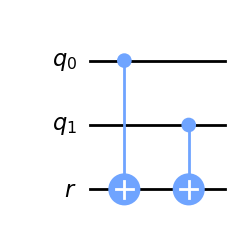
\includegraphics[width=0.5\linewidth]{XOR Cuantica.png}
    \caption{XOR Cuántica}
    \label{fig:XORCuantica}
\end{figure}

La puerta AND equivaldría cuánticamente a una puerta de Toffoli (CCNOT) con $q_0$ y $q_1$ como control y $r_1$ como objetivo.

(insertar imagen de la CCNOT)


Para la segunda mitad de la tabla ($a_0=1$) tendremos que para obtener $r_1$ basta con invertir el resultado de la tabla superior, es decir aplicar una puerta NOT, por tanto a la doble puerta CNOT de la tabla anterior le añadiremos una CNOT con $a_0$ como control para obtener el valor de $r_1$ en general.

(insertar imagen de las 3 puertas CNOT)


Para el valor de $a_1$, tendremos que es $0$ únicamente cuando $q_0$ y $q_1$ son $0$ simultáneamente, por tanto equivaldría a una CCNOT, pero con los qubits de control invertidos (que se puede lograr invirtiendo $q0$ y $q_1$ aplicando una CCNOT y volviéndolos a invertir para quedar como al inicio).

(insertar imagen de las 3 puertas CCNOT)

Una forma más sencilla de ver la salida de $a_1$ es observar que valdrá $1$ cuando $2$ o $3$ de los qubits $a_0$, $q_0$ y $q_1$ valgan $1$, y valdrá $0$ en caso contrario, cuando sólamente 1 de ellos o ninguno tenga valor $0$.
Esto lo podemos representar cuánticamente como 3 puertas CCNOT con qubits de control $a_0$ y $q_0$, $a_0$ y $q_1$, $q_0$ y $q_1$ respectivamente:

(insertar imagen de las 3 puertas CCNOT)

Esto es debido a que si únicamente 2 de los 3 qubits tienen valor $1$, se activará únicamente la puerta CCNOT que los tenga como qubits de control, mientras que si están los $3$ activados, se activarán las 3 puertas CCNOT (dando como resultado $1$ en el qubit $r1$).

El circuito final de nuestra función cuántica nos quedaría de la siguiente manera:

(insertar imagen del circuito de la función suma)

$\\$

Ahora la idea es como comentábamos más arriba aplicar dicha función de forma recursiva como mostraremos en el siguiente cuadro:

\begin{center}
    \begin{tabular}{c|c|c|c|c}
        $a_0=0$ & $r_1$ &  \\
        $q_0$   & $a_1$ & $r_2$ \\
        $q_1$   & $q_1$ & $a_2$ \\
                & $q_2$ & $q_2$
    \end{tabular}
\end{center}


$f(0,q_0,q_1) = (r_1, a_1)$
$f(a_1,q_1,q_2) = (r_2, a_2)$
$f(a_2,q_2,q_3) = (r_3, a_3)$
.
.
.
$f(a_$


\section{Problemas QUBO}
(Analizar si se puede formular algo como un problema de optimización, por ejemplo minimizar la distancia entre $\frac{X}{Y}-log_2 3$ o algo similar).

\chapter{Resultados / Análisis / Comparativa / Discusión de resultados}
Es muy importante presentar los resultados de forma clara y detallada. Analizar estos resultados, presentar comparaciones con otros trabajos y/o entre las distintas soluciones que aportemos. También es muy importante analizar cuidadosamente todos estos resultados.




BUSCAR errores segun aumenta el numero de qubit
IBM: da el porcentaje de error de sus ordenadores segun numero de qubits


Shor para factorizar numero de 10 digitos añadiendo los qubit de correccion de error.
Comparo las 3 propuestas.
eso minimizara la correccion de errores

cuanta tarda en ejecutarse un problema en cada propuesta.



Ejecutar en ordenador de ibm las 3 propeustas y apuntar los tiempos de ejecucion
Profunidad = numero de puertas basicas necesarias para mi circuito

Si la mas lenta es la que tiene menos qubits, argumentar que es la mejor porque el resultado obtenido es el mas fiable.


\chapter{Conclusiones}

Las consclusiones NO pueden limitarse a hacer un repaso del trabajo, sino que deben aportar una visión clara y sintética de lo que se extrae de todo el trabajo realizado.

Probablemente no encontremos contraejemplo (si lo hicieramos ganaríamos cerca de 1 millon de dolares), pero las conclusiones interesantes aquí se basarán en comparar la viabilidad de estos métodos, la comparativa de complejidades computacionales entre métodos clásico y cuántico, número de qubits necesarios a partir de los cuales los métodos serían viables (o superarian a su contraparte clásica) etc...
\chapter{Trabajo futuro}
En un análisis autocrítico, podemos plantear todas las limitaciones del trabajo y explicar de qué manera puede mejorarse o cómo puede llegarse a los lugares que no se hayan podido alcanzar. Hay que explicar todo esto detalladamente, NO basta con un par de párrafos generales.
\begin{thebibliography}{a}

	\bibitem[Devitt(2013)]{qecb} Devitt, S. J., Munro, W. J., y Nemoto, K. (2013). Quantum error correction for beginners.
	REPORTS ON
	PROGRESS IN PHYSICS, 76, 1-35.
 
	\bibitem[Shor(1995)]{shor95} Shor, P. W. (1995). Scheme for reducing decoherence in quantum computing memory.
	Physical
	review
	A, 52(4),	2493-2496.

	\bibitem[Nielsen(2001)]{nielsenchuang} Nielsen, M. A. y Chuang, I. L. (2001). \textit{"Quantum computation and quantum
	information. 10ª ed."}. Cambridge University Press.

\end{thebibliography}
%\bibliographystyle{plain}
%\bibliography{bibliografia}
\backmatter
\appendix
\chapter{Apéndices}
Pueden incluirse tantos apéndices como sean necesarios.


Aqui probablemente añadamos cálculos más complejos (de las fórmulas de los s-ciclos entre otras).

\end{document}
